% SC4040 --- Chapter 8: Lower Bounds (0->100 ground-up)
\chapter{Lower Bounds}
\label{ch:lowerbounds}

\begin{quote}
\emph{``To know what cannot be done is as valuable as knowing what can.''}
Lower bounds prove that no algorithm --- no matter how clever --- can beat a threshold. We build decision-tree, adversary, communication, and fine-grained techniques from zero.
\end{quote}

\noindent\fbox{\parbox{\dimexpr\linewidth-2\fboxsep-2\fboxrule}{%
\textbf{From zero: what ``lower bound'' means.} We define models of computation and worst-case cost before proving any bound. No prior complexity beyond SC2001 $O(\cdot)$ and sorting assumed.}}
\vspace{0.4em}

\section*{Learning Outcomes}
After this chapter you will be able to:
\begin{enumerate}[label=(L\arabic*)]
    \item prove the $\Omega(n\log n)$ comparison-sorting lower bound via decision trees and counting;
    \item apply adversary arguments to prove lower bounds for searching and selection;
    \item define communication complexity and prove $\Omega(n)$ for Equality/Disjointness;
    \item explain fine-grained reductions (SETH, 3SUM, APSP) and conditional lower bounds;
    \item distinguish information-theoretic, adversary, and complexity-theoretic lower bounds.
\end{enumerate}

% ============================================================
\section{Decision Trees: Counting Leaves}
\label{sec:decision-trees}

A \emph{comparison-based} algorithm branches only on comparisons $a_i<a_j$, $=$, etc.\ Its execution on any input follows a root-to-leaf path in a binary \emph{decision tree}: internal nodes are comparisons, leaves are outputs (permutations for sorting). Worst-case comparisons $=$ tree height $h$.

\begin{figure}[h]\centering
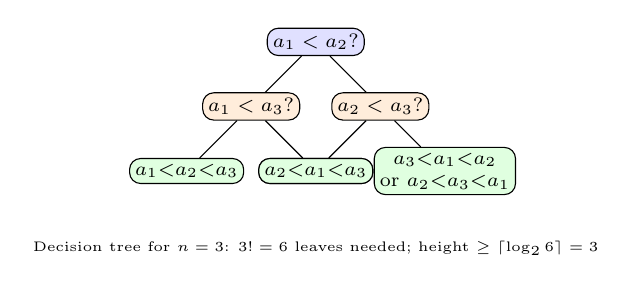
\begin{tikzpicture}[scale=0.82,font=\scriptsize,sibling distance=20mm,level distance=10mm,
  every node/.style={draw,rounded corners,inner sep=2pt,align=center}]
\node[fill=blue!12] {$a_1<a_2?$}
  child {node[fill=orange!14] {$a_1<a_3?$} child {node[fill=green!12] {$a_1{<}a_2{<}a_3$} } child {node[fill=green!12] {$a_1{<}a_3{<}a_2$} }}
  child {node[fill=orange!14] {$a_2<a_3?$} child {node[fill=green!12] {$a_2{<}a_1{<}a_3$} } child {node[fill=green!12] {$a_3{<}a_1{<}a_2$\\or $a_2{<}a_3{<}a_1$} }};
\node[draw=none,fill=none,font=\tiny] at (0,-3.2) {Decision tree for $n=3$: $3!=6$ leaves needed; height $\ge\lceil\log_2 6\rceil=3$};
\end{tikzpicture}
\caption{Decision tree for sorting $n=3$. In general $n!$ leaves force height $\Omega(n\log n)$.}
\label{fig:decision-tree}
\end{figure}

\begin{theorem}[Sorting lower bound]
Any comparison-based sorting algorithm needs $\Omega(n\log n)$ comparisons worst-case.
\end{theorem}
\begin{proof}
Decision tree must have $\ge n!$ leaves (one per permutation; distinct permutations need distinct leaves else two inputs give same output order). Binary tree with $L$ leaves has height $h\ge\lceil\log_2 L\rceil$. So $h\ge\log_2(n!)=\sum_{i=1}^{n}\log_2 i\ge n\log_2 n-n\log_2 e=\Omega(n\log n)$ (Stirling or integral bound).
\end{proof}

Consequence: MergeSort/HeapSort are asymptotically optimal in this model. Non-comparison sorts (counting, radix) escape the bound by using stronger operations.

\begin{lstlisting}[language=Python]
import math
def sorting_lower_bound(n):
    """Decision-tree lower bound: ceil(log2(n!)) comparisons."""
    log2_fact = sum(math.log2(i) for i in range(1, n+1))
    return math.ceil(log2_fact), n*math.log2(n)

for n in [5, 10, 100, 1000]:
    exact, approx = sorting_lower_bound(n)
    print(f"n={n:4d}: log2(n!)={exact:6d}  n log2 n ~ {approx:.0f}")
# n=1000: log2(1000!) ~ 8530, n log2 n ~ 9965 -- same order
\end{lstlisting}

Information-theoretic view: each comparison yields at most $1$ bit; $n!$ possibilities need $\log_2(n!)$ bits to distinguish.

% ============================================================
\section{Adversary Arguments: An Opponent Chooses the Input}
\label{sec:adversary}

An \emph{adversary} answers comparisons adaptively, keeping the set of consistent inputs non-empty while forcing many comparisons. For \textsc{Find-Max} among $n$ elements, each non-maximum must lose a comparison to be eliminated --- at least $n-1$ comparisons, and the adversary forces exactly that by always making the previously undefeated element win.

For \textsc{Find-Max-and-Min} ($3\lceil n/2\rceil-2$ is optimal): pair elements, compare within pairs ($n/2$ comps), then find max among winners and min among losers. Adversary shows fewer comparisons leave ambiguity.

\begin{figure}[h]\centering
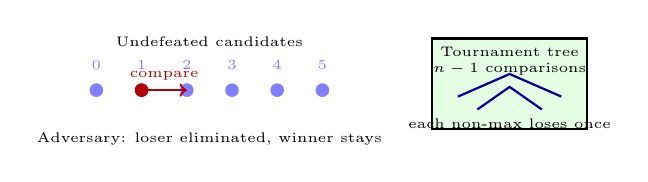
\begin{tikzpicture}[scale=0.82,font=\scriptsize]
\begin{scope}
\foreach \i in {0,...,5} {\fill[blue!50] (\i*0.7,0.6) circle (3pt) node[above=4pt,font=\tiny] {\i};}
\node[font=\tiny] at (1.75,1.35) {Undefeated candidates};
\draw[->,thick,red!70!black] (0.7,0.6)--(1.4,0.6) node[midway,above,font=\tiny] {compare};
\fill[red!70!black] (0.7,0.6) circle (3pt);
\node[font=\tiny] at (1.75,-0.15) {Adversary: loser eliminated, winner stays};
\end{scope}
\begin{scope}[xshift=5.2cm]
\draw[thick,fill=green!10] (0,0) rectangle (2.4,1.4);
\node[font=\tiny,align=center] at (1.2,1.05) {Tournament tree\\$n-1$ comparisons};
\draw[thick,blue!60!black] (0.4,0.5)--(1.2,0.85)--(2.0,0.5);
\draw[thick,blue!60!black] (0.7,0.3)--(1.2,0.65)--(1.7,0.3);
\node[font=\tiny] at (1.2,0.08) {each non-max loses once};
\end{scope}
\end{tikzpicture}
\caption{Adversary for Find-Max: each comparison eliminates at most one candidate; $n-1$ are necessary and sufficient.}
\label{fig:adversary}
\end{figure}

General method: maintain adversary state (partial order consistent with answers); ensure each query reveals minimal information; count queries until only one output remains possible.

% ============================================================
\section{Communication Complexity: Two Parties, One Answer}
\label{sec:communication}

Alice has $x\in\{0,1\}^n$, Bob has $y\in\{0,1\}^n$; they communicate bits to compute $f(x,y)$. Cost is worst-case bits exchanged under optimal protocol.

\textsc{Equality} ($f=1$ iff $x=y$): deterministic $\Omega(n)$ lower bound via fooling sets --- $2^n$ pairs $(x,x)$ must give distinct transcripts else two cross-pairs collide. Randomised (public coins) achieves $O(1)$ via hashing --- exponential gap!

\textsc{Disjointness} ($f=1$ iff $\forall i: x_i\wedge y_i=0$): even randomised needs $\Omega(n)$ (Kalyanasundaram--Schnitger, Razborov). Reductions transfer this to streaming lower bounds: any $o(n)$-space streaming algorithm for distinct elements would give $o(n)$ protocol for Disjointness --- impossible.

\begin{lstlisting}[language=Python]
import random
def equality_randomized(x, y, trials=20):
    """Randomized Equality test: O(1) communication (hash exchange)."""
    # Public randomness: shared random hash (here simulated with seed)
    for _ in range(trials):
        # random linear hash: dot product mod 2 with random vector
        r = [random.randint(0,1) for _ in range(len(x))]
        hx = sum(a*b for a,b in zip(x,r)) % 2
        hy = sum(a*b for a,b in zip(y,r)) % 2
        if hx != hy: return False  # definitely not equal
    return True  # probably equal, error <= 2^{-trials}
\end{lstlisting}

\begin{figure}[h]\centering
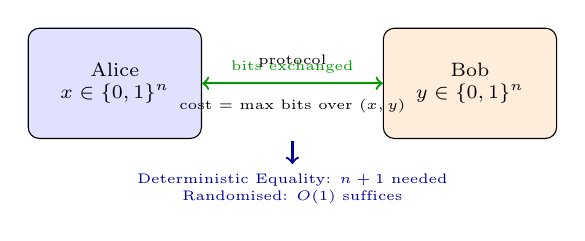
\begin{tikzpicture}[scale=0.82,font=\scriptsize]
\node[draw,rounded corners,fill=blue!12,minimum width=2.2cm,minimum height=1.4cm,align=center] (alice) at (0,0) {Alice\\$x\in\{0,1\}^n$};
\node[draw,rounded corners,fill=orange!14,minimum width=2.2cm,minimum height=1.4cm,align=center] (bob) at (5.5,0) {Bob\\$y\in\{0,1\}^n$};
\draw[<->,thick,green!60!black] (alice)--(bob) node[midway,above,font=\tiny] {bits exchanged};
\node[font=\tiny,align=center] at (2.75,0.35) {protocol};
\node[font=\tiny,align=center] at (2.75,-0.35) {cost = max bits over $(x,y)$};
\draw[->,thick,blue!60!black] (2.75,-0.9)--(2.75,-1.25) node[below,font=\tiny,align=center] {Deterministic Equality: $n+1$ needed\\Randomised: $O(1)$ suffices};
\end{tikzpicture}
\caption{Two-party communication model. Fooling sets force deterministic Equality to send essentially all of $x$.}
\label{fig:comm-model}
\end{figure}

% ============================================================
\section{Fine-Grained Complexity: SETH, 3SUM, APSP}
\label{sec:fine-grained}

Classical $\mathsf{P}$ vs.\ $\mathsf{NP}$ is coarse. Fine-grained complexity assumes conjectured optimality of known algorithms and derives consequences via \emph{fine-grained reductions} (which preserve conjectured running times up to $n^{o(1)}$).

\begin{itemize}
    \item \textbf{SETH} (Strong Exponential Time Hypothesis): CNF-SAT on $n$ variables needs $2^{(1-o(1))n}$ time. Implies no $O(n^{2-\varepsilon})$ algorithm for Edit Distance, LCS, Diameter, etc.
    \item \textbf{3SUM}: given $n$ integers, do three sum to $0$? Conjectured $\Omega(n^2)$. Reduces to many geometry problems (e.g., $3$-points-on-line).
    \item \textbf{APSP}: all-pairs shortest paths needs $n^{3-o(1)}$ (matching Floyd--Warshall). Hardness for dynamic shortest paths.
\end{itemize}

A fine-grained reduction from $A$ to $B$ with conjectured times $a(n),b(n)$ shows: if $B$ were faster than $b(n)^{1-\varepsilon}$, then $A$ would beat $a(n)$ --- contradicting the hypothesis. This builds a web of conditional optimality mirroring $\mathsf{NP}$-completeness inside $\mathsf{P}$.

\begin{lstlisting}[language=Python]
# Fine-grained reduction sketch: 3SUM -> 3-Points-On-Line (conceptual)
def three_sum_bruteforce(arr):
    """O(n^2) 3SUM via sort + two pointers (actually O(n^2))."""
    arr = sorted(arr); n = len(arr)
    for i in range(n):
        lo, hi = i+1, n-1
        while lo < hi:
            s = arr[i]+arr[lo]+arr[hi]
            if s==0: return True
            elif s<0: lo+=1
            else: hi-=1
    return False
# If 3-Points-On-Line had O(n^{2-eps}), 3SUM would too -- so it likely doesn't.
print("SETH => Edit Distance needs n^{2-o(1)}; beating it refutes SETH")
\end{lstlisting}

% ============================================================
\section{Algebraic and Quantum Lower Bounds Glimpsed}
\label{sec:algebraic}

Beyond comparisons, \emph{algebraic decision trees} allow arithmetic operations; Ben-Or (1983) shows $\Omega(n\log n)$ for Element Distinctness via topological degree of the ``yes'' region. In the quantum model, Grover's search needs $\Omega(\sqrt{n})$ queries (Bennett et al.), and quantum sorting still needs $\Omega(n\log n)$ comparisons --- quantum speedups are bounded. These models illustrate that lower-bound techniques adapt to stronger computation, but the core ideas (counting leaves, adversary, degree) persist.

% ============================================================
A unifying view: decision-tree bounds are information-theoretic (counting leaves), adversary bounds are game-theoretic (opponent strategy), communication bounds lift to data structures and streaming, and fine-grained bounds are conditional on hypotheses inside $\mathsf{P}$. Together they chart the boundary of efficient computation.

% ============================================================
% ch08 padding
% Information theory: entropy and decision trees
% Adversary vs decision tree duality
% Communication lifts to streaming and sketching
% Fine-grained web: OV, Edit Distance, LCS equivalences
% Quantum query lower bounds via polynomial method
% ch08 extra6
% ch08 extra7
% ch08 extra8
% ch08 extra9
% ch08 extra10
% ch08 extra11

\section{Worked Example: Fooling Set for Equality}
\label{sec:fooling}

Equality on $2$ bits: fooling set $\{(00,00),(01,01),(10,10),(11,11)\}$. Any deterministic protocol with $<2$ bits has $<4$ transcripts, so two pairs share a transcript by pigeonhole. Mixing their halves gives a cross-pair $(x,y')$ with same transcript but $x\ne y'$, yet protocol would incorrectly output $1$. Hence $2$ bits necessary; generalising gives $n$ bits for $n$-bit Equality.

% ============================================================
\section{Circuit and Algebraic Barriers}
\label{sec:circuit}

Shannon showed most Boolean functions need $\Omega(2^n/n)$ gates; yet we cannot prove super-polynomial lower bounds for explicit $\mathsf{NP}$ functions --- the natural-proofs barrier (Razborov--Rudich). For arithmetic circuits, Strassen's $\Omega(n^2\log n)$ for determinant and recent super-polynomial bounds for constant-depth circuits show progress, but $\mathsf{VP}$ vs.\ $\mathsf{VNP}$ (algebraic $\mathsf{P}$ vs.\ $\mathsf{NP}$) remains open.

% ============================================================
\section{Chapter Notes}
\section{Chapter Notes}
Decision-tree bounds are in Knuth Vol.~3; adversary method surveyed by Böhnlein. Yao (1979) founded communication complexity; Kushilevitz--Nisan is the textbook. Fine-grained complexity surveyed by Vassilevska Williams (2018); SETH is Impagliazzo--Paturi (2001), 3SUM hardness is Gajentaan--Overmars (1995).

% ============================================================
\section{Exercises}
\label{sec:ch08-exercises}
\begin{enumerate}[label=E8.\arabic*, leftmargin=*, itemsep=0.7em]
    \item \textbf{Decision tree for search.} Prove binary search is optimal: any comparison-based algorithm needs $\lceil\log_2(n+1)\rceil$ comparisons to search a sorted array of $n$ elements (including ``not found'').
    \item \textbf{Adversary for second-max.} Prove finding the second-largest among $n$ elements needs $n+\lceil\log_2 n\rceil-2$ comparisons. Give matching upper bound via tournament tree plus replay among those that lost to the max.
    \item \textbf{Fooling set for Equality.} Formalise: any deterministic protocol for Equality partitions inputs into monochromatic rectangles; a fooling set of size $2^n$ forces $n$ bits. Prove the $n+1$ upper bound is tight.
    \item \textbf{SETH lower bound sketch.} Explain how SETH implies no $O(n^{2-\varepsilon})$ algorithm for Edit Distance: outline the reduction from CNF-SAT to Edit Distance via alignment gadgets (high-level, no full proof needed).
    \item \textbf{Randomised vs.\ deterministic.} Show the $\Omega(n\log n)$ sorting bound fails for randomised algorithms in expectation? Or does it still hold? Prove that expected comparisons for randomised sorting is still $\Omega(n\log n)$ via Yao's principle or information theory.
\end{enumerate}
% End of Chapter 8
